\documentclass[utf8, xcolor=pst]{beamer}

%\usepackage{default}
%\usepackage{beamerthemesplit}
%\usepackage{beamerthemeAnnArbor}
% \usepackage{beamerthemeAntibes}
% \usepackage{beamerthemeBergen}
% \usepackage{beamerthemeBerkeley}
% \usepackage{beamerthemeBerlin}
% \usepackage{beamerthemeBoadilla}
% \usepackage{beamerthemeboxes}
% \usepackage{beamerthemeCambridgeUS}
% \usepackage{beamerthemeCopenhagen}
% \usepackage{beamerthemeDarmstadt}
% \usepackage{beamerthemedefault}
% \usepackage{beamerthemeDresden}
% \usepackage{beamerthemeFrankfurt}
% \usepackage{beamerthemeGoettingen}
% \usepackage{beamerthemeHannover}
% \usepackage{beamerthemeIlmenau}
% \usepackage{beamerthemeJuanLesPins}
% \usepackage{beamerthemeLuebeck}
% \usepackage{beamerthemeMadrid}
% \usepackage{beamerthemeMalmoe}
% \usepackage{beamerthemeMarburg}
% \usepackage{beamerthemeMontpellier}
% \usepackage{beamerthemePaloAlto}
% \usepackage{beamerthemePittsburgh}
% \usepackage{beamerthemeRochester}
% \usepackage{beamerthemeSingapore}
% \usepackage{beamerthemeSzeged}
% \usepackage{beamerthemeWarsaw}
\usepackage{beamerthemeFreiburg}

%\usepackage{pstricks}
\usepackage{german}
\usepackage{ragged2e}

%% zum Drucken:
% \usepackage{pgfpages}
% \pgfpagesuselayout{resize to}[a4paper,border shrink=5mm,landscape]
% \pgfpagesuselayout{2 on 1}[a4paper,border shrink=5mm]
% \pgfpagesuselayout{4 on 1}[a4paper,border shrink=5mm,landscape]
% \pgfpagesuselayout{8 on 1}[a4paper,border shrink=5mm]
% \pgfpagesuselayout{16 on 1}[a4paper,border shrink=5mm,landscape]


\title[Ethersex]{Das Ethersex-Projekt}
\subtitle{Einführung}
\author[RayVey]{Rayhope \and Veyron\newline \texttt{ethersex-devel@list.zerties.org}}
\date[LaTa ’09]{Labortage '09 \\ \texttt{Prickle-Prickle, The Aftermath 12, 3175 YOLD}}

\titlegraphic{
\includegraphics[width=0.5cm]{gnu-fdl.png}}
\logo{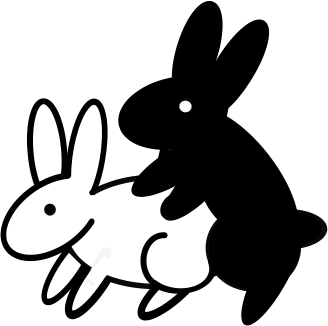
\includegraphics[width=1.5cm]{./bunnies-bg.png}}
% \logo{\pgfimage[width=1.5cm]{bunnies.png}}


\begin{document}

\frame{
  \frametitle{Ein Kurzvortrag}
  \titlepage
}

\section[Inhalt]{}
\frame{
  \frametitle{Übersicht}
  \tableofcontents[pausesections]
}

\section{Einleitung}
 \frame{
  \frametitle{Einleitung}
  \begin{block}<1->{Zitat}
    \begin{quote}
      \justifying{
	Der Urquell aller technischen Errungenschaften
	ist die göttliche Neugier und der Spieltrieb des bastelnden und grübelnden Forschers
	und nicht minder die konstruktive Fantasie des technischen Erfinders...\\
	(A. Einstein: Eröffnung IFA 1930)
      }
    \end{quote}
  \end{block}
  \begin{block}<2->{Zusatz}
    \begin{quote}
      \justifying{
	... und Softwareentwicklers.
      }
    \end{quote}
  \end{block}
}

\subsection{Historie}
\frame{
  \frametitle{Die Entstehungsgeschichte}
  \begin{block}{Die Anfänge}
    \begin{itemize}
      \item<1-> fd0 startet Softwareprojekt für die Hardware Etherrape
      \item<2-> Stesie implementiert IPv6.
      \item<3-> Stettberger baut RFM12 ein.
    \end{itemize}
  \end{block}
}

\section{Module}
\frame{
  \frametitle{Die Module}
  \begin{block}<1->{Vielfalt}
    \begin{itemize}
      \item<1-> Netzwerkanbindung
      \item<1-> Interaktion mit dem Anwender
      \item<1-> Netzwerkprotokolle
      \item<1-> Kontakt zur Außenwelt
      \item<1-> Verschiedenes
    \end{itemize}
  \end{block}
  \begin{block}<2->{Komfort}
    \begin{itemize}
      \item<2-> Menü gesteuerte Auswahl der Module
      \begin{itemize}
	\item<3-> keine unötiger Overhead
      \end{itemize}
    \end{itemize}
  \end{block}
  \begin{block}<4->{Einfach}
    \begin{itemize}
      \item<4-> Modulare Einbindung eigener Features
    \end{itemize}
  \end{block}
}
\subsection{Modulübersicht}
% \subsubsection{Netzwerk-anbindung}
\frame{
\frametitle{Ethersex features}
\begin{block}{Netzwerkanbindung}
\begin{itemize}
  \item Ethernet (ENC28J60) inkl. IEEE 802.1q (VLANs)
  \item USB (Software USB, Userland TUN Treiber)
  \item RFM12 (Funkübertragung auf dem 433 MHz ISM-Band)
  \item ZBus - Eigenes Protokoll für serielle Schnittstelle
\end{itemize}
\end{block}
}

% \subsubsection{Interaktion mit dem Anwender}
%% \frame{
%% \frametitle{Ethersex features}
%% \begin{block}{Interaktion mit dem Anwender}
%% \begin{itemize}
%%   \item HTTP-Server (mit Zugriff auf Dateien und ECMD)
%%   \item text-basiert (Telnet-ähnlich, TCP/IP oder UDP/IP)
%%   \item über serielle Schnittstelle
%%   \item über I2C
%%   \item via Jabber/XMPP
%%   \item via IRC
%% \end{itemize}
%% \end{block}
%% }

% \subsubsection{Netzwerkprotokolle}
\frame{
\frametitle{Ethersex features}
\begin{block}{Netzwerkprotokolle}
\begin{itemize}
  \item TCP/IP, UDP/IP und ICMP
  \item BOOTP (einfacherer, besser geeigneterer, Vorgänger von DHCP, der jedoch von allen gängigen DHCP-Servern unterstützt wird)
  \item TFTP (Upload von Firmwaredateien bzw. in den Data Flash Baustein)
  \item SYSLOG
  \item SNMP
  \item SMTP (E-Mail-Versand)
  \item NTP (Client und Server)
  \item DNS
\end{itemize}
\end{block}
}
\frame{
\frametitle{Ethersex features}
\begin{block}{Netzwerkprotokolle}
\begin{itemize}
  \item mDNS (Avahi)
  \item DynDNS
  \item MySQL (Client)
  \item IRC (Client)
  \item MPD (Music Player Daemon; einfache Steuerungsaufgaben)
  \item SOAP/XMLRPC
  \item UPnP
\end{itemize}
\end{block}
}

% \subsubsection{Kontakt zur Außenwelt}
% \frame[allowframebreaks]{
\frame{
\frametitle{Ethersex features}
\begin{block}{Kontakt zur Außenwelt}
\begin{itemize}
  \item RS232 und RS485
  \item Infrarotsender und -empfänger (RC5 Fernbedienungen!)
  \item I2C (Master und Slave)
  \item Steuerung von FS20-Modulen (Funkmodule von ELV bzw. Conrad, u.a. Steckdosen, Dimmer und Temperatursensoren)
  \item Modbus
  \item YPort (Serial over LAN (SOL) auch als XPort bekannt)
  \item Blinkenlights MCUF
  \item Porterweiterungen durch HC595 und HC165 möglich
\end{itemize}
\end{block}
}
\frame{
\frametitle{Ethersex features}
\begin{block}{Kontakt zur Außenwelt}
\begin{itemize}
  \item Dateneingabe mittels PS/2 Tastatur
  \item Dallas 1-wire Bus
  \item LCD (HD44780 und Kompatible)
  \item Philips dc3840 camera und MCA25-Handycam
  \item Stella Light (PWM für bis zu 8 Kanäle)
  \item Senertec Dachs MSR1 auslesen
  \item SMS
\end{itemize}
\end{block}
}

% \subsubsection{Verschiedenes}
\frame{
\frametitle{Ethersex features}
\begin{block}{Verschiedenes}
\begin{itemize}
  \item Fernsteuern von vielen Funksteckdosen mit RFM12 ASK
  \item Atmel DataFlash (SPI Flash)
  \item MMC/SD-Kartenleser
  \item Sound
  \item PAM Schicht zur Authentifizierung (z.b. ECMD-TCP)
  \item Systemuhr
  \item CRON-Dienst (analog dem crond auf Unix-Systemen)
  \item Pins können mit symbolischen Namen versehen werden
\end{itemize}
\end{block}
}
\frame{
\frametitle{Ethersex features}
\begin{block}{Verschiedenes}
\begin{itemize}
  \item Control6
  \item AliasCmd/Alias Namen für Befehle
  \item ECMD Scripting
  \item Virtuelles Dateisystem für DataFlash, MMC/SD-Karten und EEPROMs
  \item Netstat/Online Statistik
\end{itemize}
\end{block}
}



\subsection{Einstellen}
\frame{
  \frametitle{Modulauswahl}
  Menuconfig: Hauptfenster
  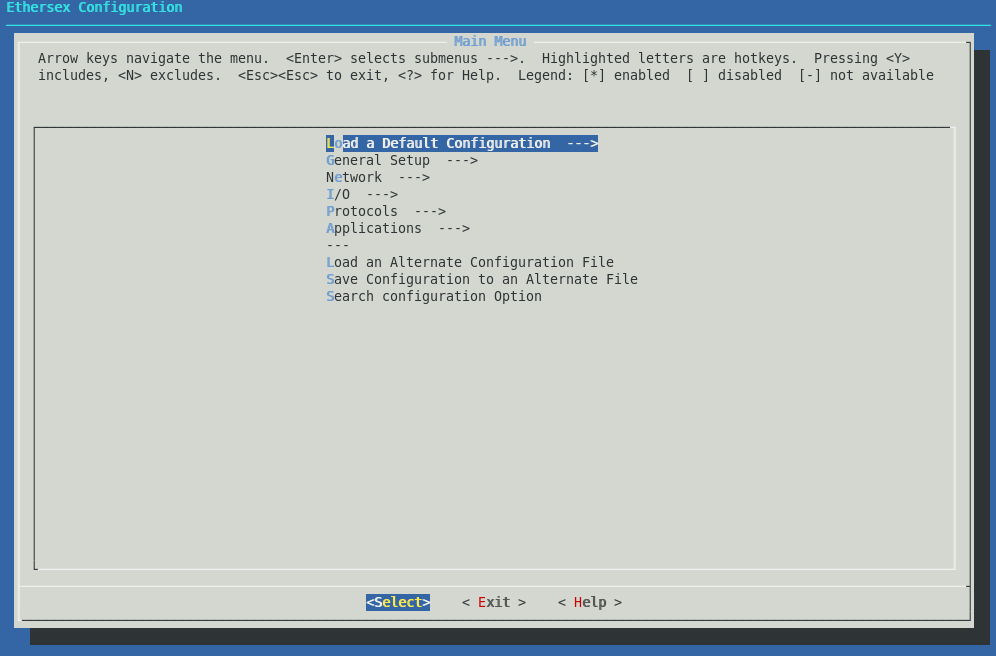
\includegraphics[width=10cm]{Main.png}
}
\frame{
  \frametitle{Modulauswahl}
  Menuconfig: Generelle Einstellungen
  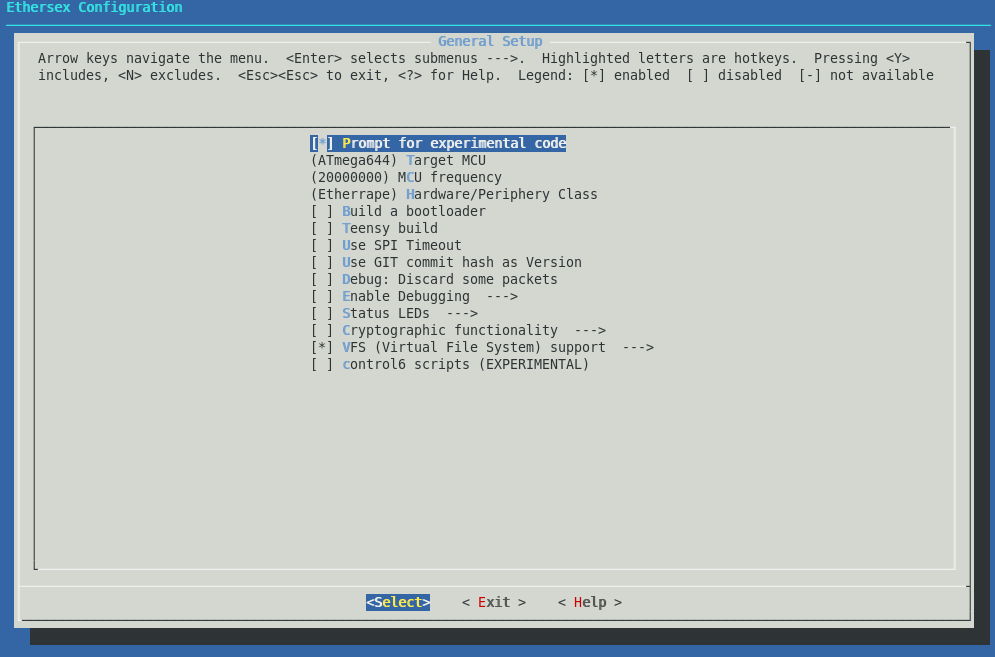
\includegraphics[width=10cm]{General.png}
}

\subsection{Hinzufügen}
\frame{
  \frametitle{Eigene Module hinzufügen}
Metaschicht?\\
Control6?
}

\section{Hardware}
\frame{
  \frametitle{Zielplatform}
  \begin{block}<1->{Vielfalt}
    \begin{itemize}
      \item<1-> Prozessor: AVR Atmega
      \begin{itemize}
	\item<2-> Bausätze
	\item<3-> Eigenbau
      \end{itemize}
    \end{itemize}
  \end{block}
  \begin{block}<4->{Komfort}
    \begin{itemize}
      \item<4-> Menü gesteuerte Auswahl der Hardware
    \end{itemize}
  \end{block}
  \begin{block}<5->{Einfach}
    \begin{itemize}
      \item<5-> Skriptgeführte Erstellung der Konfigurationsdateien
    \end{itemize}
  \end{block}
}

\subsection{Unterstütze Hardware}
\frame{
  \frametitle{Unterstütze Hardware}
  \begin{block}<1->{Bausätze}
    \begin{itemize}
      \item Etherrape (fd0;lochraster.org)
      \item Net-IO (Pollin)
      \item AVR-Webserver (U. Radig)
      \item Thermotronic Basic (Eurotronic) \\Thermy (Aldi)
      \item ProBot (Conrad)
      \item ...
    \end{itemize}
  \end{block}

  \begin{block}<2->{Eigenbau}
    \begin{itemize}
      \item Bettwächter (stesie; zerties.org)
      \item ...
    \end{itemize}
  \end{block}
}

\subsection{Eigenen Hardware}
\frame{
  \frametitle{Eigenen Hardware}
Hackery?\\
add-hardwarebrocken.sh?
}

\section{Fragen}
\frame{
\frametitle{www.ethersex.de}
Fragen? \\
Anregungen? \\
\bigskip 
\bigskip 
\bigskip 
\begin{center}
\textbf{Danke für die Aufmerksamkeit!}\end{center}
\bigskip 
\bigskip 
\bigskip 
\begin{center}
 \begin{small}Projekt-Wiki: \texttt{www.ethersex.de}\\ Vortragsfolien: \texttt{www.ethersex.de/index.php/Kurzvortrag} \end{small}
\end{center}
}
\end{document}
